\begin{frame}[fragile]
  \frametitle{Funciones}

  Una funci\'on es un fragmento de c\'odigo con un nombre asociado que
  realiza una serie de tareas y devuelve un valor.

  \begin{itemize}
  \item{Ejemplo:}
  \end{itemize}
  
  \begin{figure}
    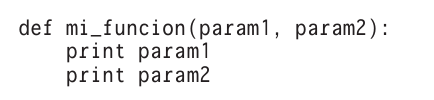
\includegraphics[width=0.6\textwidth]{Imagenes/Ejm.jpg}
    \caption{\label{fig:Ejm}Esta funci\'on imprime los dos par\'ametros ingresados.}
  \end{figure}

\end{frame}
